\documentclass[12pt, titlepage]{article}

\usepackage{fullpage}
\usepackage[round]{natbib}
\usepackage{multirow}
\usepackage{booktabs}
\usepackage{tabularx}
\usepackage{graphicx}
\usepackage{float}
\usepackage{xr}
\usepackage{hyperref}
\hypersetup{
    colorlinks,
    citecolor=blue,
    filecolor=black,
    linkcolor=red,
    urlcolor=blue
}
\externaldocument{../../SRS/SRS}
%% Comments

\usepackage{color}

\newif\ifcomments\commentstrue

\ifcomments
\newcommand{\authornote}[3]{\textcolor{#1}{[#3 ---#2]}}
\newcommand{\todo}[1]{\textcolor{red}{[TODO: #1]}}
\else
\newcommand{\authornote}[3]{}
\newcommand{\todo}[1]{}
\fi

\newcommand{\wss}[1]{\authornote{blue}{SS}{#1}} 
\newcommand{\wxz}[1]{\authornote{cyan}{XZ}{#1}} 
\newcommand{\plt}[1]{\authornote{magenta}{TPLT}{#1}} %For explanation of the template
\newcommand{\an}[1]{\authornote{cyan}{Author}{#1}}

%% Common Parts

\newcommand{\progname}{ProgName} % PUT YOUR PROGRAM NAME HERE %Every program
                                % should have a name


\newcounter{acnum}
\newcommand{\actheacnum}{AC\theacnum}
\newcommand{\acref}[1]{AC\ref{#1}}

\newcounter{ucnum}
\newcommand{\uctheucnum}{UC\theucnum}
\newcommand{\uref}[1]{UC\ref{#1}}

\newcounter{mnum}
\newcommand{\mthemnum}{M\themnum}
\newcommand{\mref}[1]{M\ref{#1}}

\begin{document}

\title{Module Guide for RSSC} 
\author{Xingzhi Liu}
\date{\today}

\maketitle

\pagenumbering{roman}

\section{Revision History}

\begin{tabularx}{\textwidth}{p{3cm}p{2cm}X}
\toprule {\bf Date} & {\bf Version} & {\bf Notes}\\
\midrule
Nov 19, 2020 & 1.0 & First Draft\\
Dec 18, 2020 & 1.1 & Revision 1\\
\bottomrule
\end{tabularx}

\newpage

\section{Reference Material}

This section records information for easy reference.

\subsection{Abbreviations and Acronyms}

\renewcommand{\arraystretch}{1.2}
\begin{tabular}{l l} 
  \toprule		
  \textbf{symbol} & \textbf{description}\\
  \midrule 
  AC & Anticipated Change\\
  DAG & Directed Acyclic Graph \\
  M & Module \\
  MG & Module Guide \\
  OS & Operating System \\
  R & Requirement\\
  SC & Scientific Computing \\
  SRS & Software Requirements Specification\\
  RSSC & Explanation of program name\\
  UC & Unlikely Change \\
  \bottomrule
\end{tabular}\\

\newpage

\tableofcontents

\listoftables

\listoffigures

\newpage

\pagenumbering{arabic}

\section{Introduction}

Decomposing a system into modules is a commonly accepted approach to developing
software.  A module is a work assignment for a programmer or programming
team~\citep{ParnasEtAl1984}.  We advocate a decomposition
based on the principle of information hiding~\citep{Parnas1972a}.  This
principle supports design for change, because the ``secrets'' that each module
hides represent likely future changes.  Design for change is valuable in SC,
where modifications are frequent, especially during initial development as the
solution space is explored.  

Our design follows the rules layed out by \citet{ParnasEtAl1984}, as follows:
\begin{itemize}
\item System details that are likely to change independently should be the
  secrets of separate modules.
\item Each data structure is implemented in only one module.
\item Any other program that requires information stored in a module's data
  structures must obtain it by calling access programs belonging to that module.
\end{itemize}

After completing the first stage of the design, the Software Requirements
Specification (SRS), the Module Guide (MG) is developed~\citep{ParnasEtAl1984}. The MG
specifies the modular structure of the system and is intended to allow both
designers and maintainers to easily identify the parts of the software.  The
potential readers of this document are as follows:

\begin{itemize}
\item New project members: This document can be a guide for a new project member
  to easily understand the overall structure and quickly find the
  relevant modules they are searching for.
\item Maintainers: The hierarchical structure of the module guide improves the
  maintainers' understanding when they need to make changes to the system. It is
  important for a maintainer to update the relevant sections of the document
  after changes have been made.
\item Designers: Once the module guide has been written, it can be used to
  check for consistency, feasibility and flexibility. Designers can verify the
  system in various ways, such as consistency among modules, feasibility of the
  decomposition, and flexibility of the design.
\end{itemize}

The rest of the document is organized as follows. Section
\ref{SecChange} lists the anticipated and unlikely changes of the software
requirements. Section \ref{SecMH} summarizes the module decomposition that
was constructed according to the likely changes. Section \ref{SecConnection}
specifies the connections between the software requirements and the
modules. Section \ref{SecMD} gives a detailed description of the
modules. Section \ref{SecTM} includes two traceability matrices. One checks
the completeness of the design against the requirements provided in the SRS. The
other shows the relation between anticipated changes and the modules. Section
\ref{SecUse} describes the use relation between modules.

\section{Anticipated and Unlikely Changes} \label{SecChange}

This section lists possible changes to the system. According to the likeliness
of the change, the possible changes are classified into two
categories. Anticipated changes are listed in Section \ref{SecAchange}, and
unlikely changes are listed in Section \ref{SecUchange}.

\subsection{Anticipated Changes} \label{SecAchange}

Anticipated changes are the source of the information that is to be hidden
inside the modules. Ideally, changing one of the anticipated changes will only
require changing the one module that hides the associated decision. The approach
adapted here is called design for
change.

\begin{description}
\item[\refstepcounter{acnum} \actheacnum \label{acHardware}:] The specific
  hardware on which the software is running.
\item[\refstepcounter{acnum} \actheacnum \label{acControl}:] The overall control of the calculation. (e.g. shall we calculate the signal strength at different sampling points in parallel or calculate them one by one?)
\item[\refstepcounter{acnum} \actheacnum \label{acInputParam}:] The format of the
  input parameters.
\item[\refstepcounter{acnum} \actheacnum \label{acInputConstr}:] The constraints on the
  input parameters.
\item[\refstepcounter{acnum} \actheacnum \label{acOutputParam}:] The format of the
  output data.
\item[\refstepcounter{acnum} \actheacnum \label{acSignalCompose}:] What composes the received signal at the sampling point(e.g. direct signal, reflection, refraction, diffraction... What shall we consider in our calculation and what shall we neglect?).
\item[\refstepcounter{acnum} \actheacnum \label{acDirectLoss}:] How the radio propagation loss models with direct paths are defined using the input parameters.
\item[\refstepcounter{acnum} \actheacnum \label{acIntersection}:] How the intersections of line segments are detected.
\item[\refstepcounter{acnum} \actheacnum \label{acPathSegments}:] How the linear segments of first-order reflected signals' paths are found. 
\end{description}

\subsection{Unlikely Changes} \label{SecUchange}

The module design should be as general as possible. However, a general system is
more complex. Sometimes this complexity is not necessary. Fixing some design
decisions at the system architecture stage can simplify the software design. If
these decision should later need to be changed, then many parts of the design
will potentially need to be modified. Hence, it is not intended that these
decisions will be changed.

\begin{description}
\item[\refstepcounter{ucnum} \uctheucnum \label{ucIO}:] Input/Output files
  (Input files: three files in .csv format: tsmFile for transmitter, spFile for sampling points, and wallFile for the floor map; Output file: one file in .csv format).
\item[\refstepcounter{ucnum} \uctheucnum \label{ucWallShape}:] Walls are linear with finite lengths.
\item[\refstepcounter{ucnum} \uctheucnum \label{ucSingleSource}:] Only one transmitter works in the area of simulation.
\item[\refstepcounter{ucnum} \uctheucnum \label{ucSegment}:] Line segments are represented with a starting and an ending point, in addition to the linear equation (e.g. $m1\cdot x+m2\cdot y = k$) of that line.
\item[\refstepcounter{ucnum} \uctheucnum \label{ucEquation}:] A linear equation $m1\cdot x+m2\cdot y = k$ will be represented as a series of 3 parameters: $m1, m2,$ and $k$ in RSSC. 
\item[\refstepcounter{ucnum} \uctheucnum \label{ucOutputConstr}:] The constraints on the output data will not not change due to the law of conservation of energy. 
\end{description}

\section{Module Hierarchy} \label{SecMH}

This section provides an overview of the module design. Modules are summarized
in a hierarchy decomposed by secrets in Table \ref{TblMH}. The modules listed
below, which are leaves in the hierarchy tree, are the modules that will
actually be implemented.

\begin{description}
\item [\refstepcounter{mnum} \mthemnum \label{mHH}:] Hardware-Hiding Module
\item [\refstepcounter{mnum} \mthemnum \label{mIP}:] Input Parameters
\item [\refstepcounter{mnum} \mthemnum \label{mO}:] Output
\item [\refstepcounter{mnum} \mthemnum \label{mCM}:] Control Module
\item [\refstepcounter{mnum} \mthemnum \label{mRS}:] Received Signal
\item [\refstepcounter{mnum} \mthemnum \label{mSPM}:] Specification Parameters Module
\item [\refstepcounter{mnum} \mthemnum \label{mP}:] Point
\item [\refstepcounter{mnum} \mthemnum \label{mW}:] Wall
\item [\refstepcounter{mnum} \mthemnum \label{mFM}:] Input Floor Map
\item [\refstepcounter{mnum} \mthemnum \label{mEF}:] Equation Finder
\item [\refstepcounter{mnum} \mthemnum \label{mLSP}:] Linear Signal Path
\item [\refstepcounter{mnum} \mthemnum \label{mI}:] Intersection
\item [\refstepcounter{mnum} \mthemnum \label{mLPL}:] Linear Path Loss
\item [\refstepcounter{mnum} \mthemnum \label{mLOS}:] Line-Of-Sight Signal
\item [\refstepcounter{mnum} \mthemnum \label{mSR}:] Specular Reflection
\item [\refstepcounter{mnum} \mthemnum \label{mFORS}:] First-Order Reflection
\end{description}


\begin{table}[h!]
\centering
\begin{tabular}{p{0.3\textwidth} p{0.6\textwidth}}
\toprule
\textbf{Level 1} & \textbf{Level 2}\\
\midrule

{Hardware-Hiding Module} & ~ \\
\midrule

\multirow{3}{0.3\textwidth}{Behaviour-Hiding} & Input Parameters\\
& Output\\
& Control Module\\
& Specification Parameters\\
\midrule

\multirow{3}{0.3\textwidth}{Software Decision} & Point\\
& Wall\\
& Floor Map\\
& Equation Finder\\
& Linear Signal Path\\
& Intersection\\
& Linear Path Loss\\
& Line-Of-Sight Signal\\
& Specular Reflection\\
& First Order Reflection Signal\\
& Received Signal Strength\\
\bottomrule

\end{tabular}
\caption{Module Hierarchy}
\label{TblMH}
\end{table}

\section{Connection Between Requirements and Design} \label{SecConnection}

The design of the system is intended to satisfy the requirements developed in
the SRS. In this stage, the system is decomposed into modules. The connection
between requirements and modules is listed in Table \ref{TblRT}.

\section{Module Decomposition} \label{SecMD}

Modules are decomposed according to the principle of ``information hiding''
proposed by \citet{ParnasEtAl1984}. The \emph{Secrets} field in a module
decomposition is a brief statement of the design decision hidden by the
module. The \emph{Services} field specifies \emph{what} the module will do
without documenting \emph{how} to do it. For each module, a suggestion for the
implementing software is given under the \emph{Implemented By} title. If the
entry is \emph{OS}, this means that the module is provided by the operating
system or by standard programming language libraries.  \emph{RSSC} means the
module will be implemented by the RSSC software.

Only the leaf modules in the hierarchy have to be implemented. If a dash
(\emph{--}) is shown, this means that the module is not a leaf and will not have
to be implemented.

\subsection{Hardware Hiding Modules (\mref{mHH})}

\begin{description}
\item[Secrets:]The data structure and algorithm used to implement the virtual
  hardware.
\item[Services:]Serves as a virtual hardware used by the rest of the
  system. This module provides the interface between the hardware and the
  software. So, the system can use it to display outputs or to accept inputs.
\item[Implemented By:] OS
\end{description}

\subsection{Behaviour-Hiding Module}

\begin{description}
\item[Secrets:]The contents of the required behaviours.
\item[Services:]Includes programs that provide externally visible behaviour of
  the system as specified in the software requirements specification (SRS)
  documents. This module serves as a communication layer between the
  hardware-hiding module and the software decision module. The programs in this
  module will need to change if there are changes in the SRS.
\item[Implemented By:] --
\end{description}

\subsubsection{Input Parameters Module (\mref{mIP})}

\begin{description}
\item[Secrets:]The data structure for input parameters, how the values are input and verified.
\item[Services:]Gets input from user, verifies that the inputs meet the physical and software constraints, and stores input for other modules to read.
\item[Implemented By:] RSSC
\end{description}

\subsubsection{Output Module (\mref{mO})}

\begin{description}
\item[Secrets:]The format and structure for output data.
\item[Services:]Outputs calculation results to a text file.
\item[Implemented By:] RSSC
\end{description}

\subsubsection{Control Module (\mref{mCM})}

\begin{description}
\item[Secrets:]The algorithm for coordinating the running of the program.
\item[Services:]Provide the main program.
\item[Implemented By:] RSSC
\end{description}

\subsubsection{Received Signal Strength Module (\mref{mRS})}

\begin{description}
\item[Secrets:]The solver for the received radio signal strength.
\item[Services:]Combines signals from different paths and find the total strength of the combined signal. Also verifies whether the combined signal satisfies the law of conservation of energy or not.
\item[Implemented By:] RSSC
\end{description}

\subsubsection{Specification Parameters Module (\mref{mSPM})}

\begin{description}
\item[Secrets:]The values of the specification patameters.
\item[Services:]Read access for the specification parameters.
\item[Implemented By:] RSSC
\end{description}

\subsection{Software Decision Module}

\begin{description}
\item[Secrets:] The design decision based on mathematical theorems, physical
  facts, or programming considerations. The secrets of this module are
  \emph{not} described in the SRS.
\item[Services:] Includes data structure and algorithms used in the system that
  do not provide direct interaction with the user. 
  % Changes in these modules are more likely to be motivated by a desire to
  % improve performance than by externally imposed changes.
\item[Implemented By:] --
\end{description}

\subsubsection{Point Module (\mref{mP})}

\begin{description}
\item[Secrets:]The data structure for a Point type.
\item[Services:]Provides operations of creating points, setting point position and reading point position.
\item[Implemented By:] RSSC
\end{description}

\subsubsection{Wall Module (\mref{mW})}

\begin{description}
\item[Secrets:]The data structure for a Wall type.
\item[Services:]Provides operations of creating a wall, as well as setting and reading of wall parameters including transmittance, reflectance, and starting or ending points of the wall.
\item[Implemented By:] RSSC
\end{description}

\subsubsection{Floor Map Module (\mref{mFM})}

\begin{description}
\item[Secrets:]The data structure for a Floor Map type.
\item[Services:]Provides operations of creating and reading of a Floor Map from the user input.  
\item[Implemented By:] RSSC
\end{description}

\subsubsection{Equation Finder Module (\mref{mEF})}

\begin{description}
\item[Secrets:]The algorithm to find proper linear equation representation for a line segment.
\item[Services:]Find coefficients of a line segment's linear equation from the vertices of the segment.
\item[Implemented By:] RSSC
\end{description}

\subsubsection{Linear Signal Path Module (\mref{mLSP})}

\begin{description}
\item[Secrets:]The data structure for a Linear Signal Path type.
\item[Services:]Provides operations of creating a Linear Signal Path, as well as reading of path parameters including starting and ending vertices, linear equation parameters and path length. 
\item[Implemented By:] RSSC
\end{description}

\subsubsection{Intersection Module (\mref{mI})}

\begin{description}
\item[Secrets:]The algorithm to find a signal path's intersection point on a wall.
\item[Services:]Finds the potential intersection point of the wall's line and the signal path's line and determines the validity of the intersection (whether the potential intersection point is both on the wall and on the signal path).
\item[Implemented By:] RSSC
\end{description}

\subsubsection{Linear Path Loss Module (\mref{mLPL})}

\begin{description}
\item[Secrets:]The algorithm to find the propagation loss along a linear signal path.
\item[Services:]Calculate the percentage of power that a radio signal would remain after travelling through a given linear signal path.
\item[Implemented By:] RSSC
\end{description}

\subsubsection{Line-Of-Sight Signal Module (\mref{mLOS})}

\begin{description}
\item[Secrets:]The data structure for a Line-Of-Sight Signal type.
\item[Services:]Provides operations of creating a Line-Of-Sight Signal and reading of parameters including the signal's strength and phase angle at its destination, and the length of its transmission path. 
\item[Implemented By:] RSSC
\end{description}

\subsubsection{Specular Reflection Module (\mref{mSR})}

\begin{description}
\item[Secrets:]The algorithm to find linear segments of a reflected signal path.
\item[Services:]For a signal given an origin, a destination, and a potential reflection surface, determines the linear signal path from the origin to the reflection surface, the path from the reflection surface to the destination, and the validity of the whole path.
\item[Implemented By:] RSSC
\end{description}

\subsubsection{First-Order Reflection Signal Module (\mref{mFORS})}

\begin{description}
\item[Secrets:]The data structure for a First-Order Reflection Signal type.
\item[Services:]Provides operations of creating a First-Order Reflection Signal, and reading of parameters including the signal's strength and phase angle at its destination. 
\item[Implemented By:] RSSC
\end{description}

\section{Traceability Matrix} \label{SecTM}

This section shows two traceability matrices: between the modules and the
requirements and between the modules and the anticipated changes. Two of the anticipated changes (\acref{acInputParam} and \acref{acInputConstr}) are mapped to the same module (\mref{mIP}). The reason for this is that the services to store and verify user inputs in this module will always be provided together.


\begin{table}[H]
\centering
\begin{tabular}{p{0.2\textwidth} p{0.6\textwidth}}
\toprule
\textbf{Req.} & \textbf{Modules}\\
\midrule
R\ref{R_Inputs} & \mref{mHH}, \mref{mIP}, \mref{mCM}\\
R\ref{R_VerifyInputs} & \mref{mIP}, \mref{mSPM}\\
R\ref{R_Calculate} & \mref{mRS}, \mref{mP}, \mref{mW}, \mref{mFM}, \mref{mEF}, \mref{mLSP}, \mref{mI}, \mref{mLPL}, \mref{mLOS}, \mref{mSR}, \mref{mFORS}\\
R\ref{R_VerifyOutput} & \mref{mRS}\\
R\ref{R_Output} & \mref{mO}\\
\bottomrule
\end{tabular}
\caption{Trace Between Requirements and Modules}
\label{TblRT}
\end{table}

\begin{table}[H]
\centering
\begin{tabular}{p{0.2\textwidth} p{0.6\textwidth}}
\toprule
\textbf{AC} & \textbf{Modules}\\
\midrule
\acref{acHardware} & \mref{mHH}\\
\acref{acControl} & \mref{mCM}\\
\acref{acInputParam} & \mref{mIP}\\
\acref{acInputConstr} & \mref{mIP}\\
\acref{acOutputParam} & \mref{mO}\\
\acref{acSignalCompose} & \mref{mRS}\\
\acref{acDirectLoss} & \mref{mLPL}\\
\acref{acIntersection} & \mref{mI}\\
\acref{acPathSegments} & \mref{mSR}\\
\bottomrule
\end{tabular}
\caption{Trace Between Anticipated Changes and Modules}
\label{TblACT}
\end{table}

\section{Use Hierarchy Between Modules} \label{SecUse}

In this section, the uses hierarchy between modules is
provided. \citet{Parnas1978} said of two programs A and B that A {\em uses} B if
correct execution of B may be necessary for A to complete the task described in
its specification. That is, A {\em uses} B if there exist situations in which
the correct functioning of A depends upon the availability of a correct
implementation of B.  Figure \ref{FigUH} illustrates the use relation between
the modules. It can be seen that the graph is a directed acyclic graph
(DAG). Each level of the hierarchy offers a testable and usable subset of the
system, and modules in the higher level of the hierarchy are essentially simpler
because they use modules from the lower levels.

\begin{figure}[H]
\centering
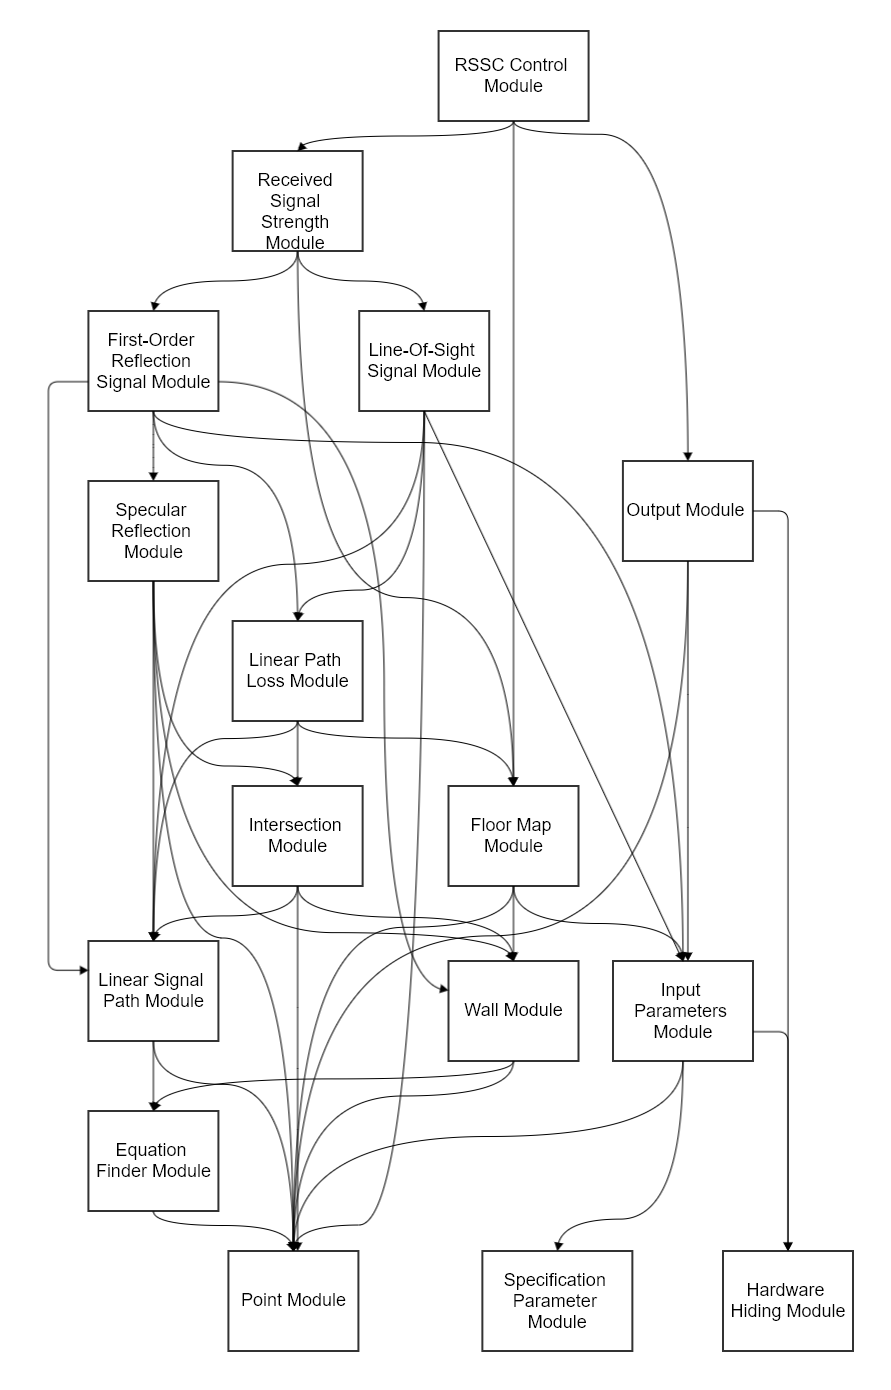
\includegraphics[width=0.9\textwidth]{uses_hierarchy.png}
\caption{Use hierarchy among modules}
\label{FigUH}
\end{figure}

%\section*{References}

\newpage
\bibliographystyle {plainnat}
\bibliography{../../../refs/References}

\end{document}